\section{The Venue Manager}

% This template is only made for the textual part of your use cases
% and doesn't replace the need for a diagram. Using this allows for
% a better understanding of how the application and functions within
% it should work.
%
% Name:
%
% Pre-conditions:
%
% Post-conditions:
%
% Purpose:
%
% Description:

% \includegraphics[width=\linewidth]{useCaseManager.png}

\subsection{Add Event}
\textbf{Pre-conditions}: The venue manager is logged in into the system.\\

\textbf{Post-conditions}: A new event exists in the system, with a start
and end date and a name.\\

\textbf{Purpose}:The venue manager wants to add an event to the ticket
selling system in order to allow customers to buy tickets for it and
to promote it.\\

\textbf{Description}: The venue manager fills in the form for the creation
of a new event with the name of the event and a description of it, then
selects a start and end date from the "calendar menus". When they are
satisfied with all the details, they press the save button and the
changes are saved in the system.

\subsection{Reschedule Event}
\textbf{Pre-conditions}:The venue manager is logged in into the system
and at least one event exists in the system that hasn't been cancelled
already\\

\textbf{Post-conditions}: An existing event has either a new start date,
a new end date or both\\

\textbf{Purpose}:The venue manager wants to change the dates an event
runs for in order to allow customers to have the accurate dates the
event will be occuring and for them to be able to buy tickets for it\\

\textbf{Description}:
The manager selects the event from a list of events, then a screen with
the event's information displayed in a form style appears, allowing the
manager to  make the changes he needs to make to the dates, then they
press the save button and the changes are saved into the system.

\subsection{Cancel Event}
\textbf{Pre-conditions}: The venue manager is logged in into the system and
at least one event exists in the system.\\

\textbf{Post-conditions}: A previously existing event will be displayed
as cancelled in the system and no more tickets will be available for sale
for that event (the event won't be deleted from the system though, in case
customers have already seen the event in the system and/or bought tickets
for it)\\

\textbf{Purpose}: The venue manager wants to cancel an event that was
scheduled to occur for any reason in order to inform the customers
that the event is no longer occuring.\\

\textbf{Description}: The venue manager selects the event they wish to
cancel from a list and then the system prompts them with a message
to confirm they wish to cancel that event. If the user selects yes, the
changes are saved into the system and the event will then appear as
cancelled to the users.

\subsection{Add Show}
\textbf{Pre-conditions}: The venue manager is logged in into the system
and at least one event exists in the system.\\

\textbf{Post-conditions}: A new showning for an event exists in the system,
with a date and start time and a maximum-seats-per-customer value.\\

\textbf{Purpose}: The venue manager wants to add a showing to an event
that is planned to inform the customers and agents of the show occurence
and allow for tickets to be sold.\\

\textbf{Description}: The manager selects the event for which they
want to add a show from a list, then enters the details of the show
in a form (date the show is happening and start and end time as well
as the maximum-seats-per-customer value) and then presses save which
will save the changes in the system and inform the user of the changes.

\subsection{Reschedule Show}
\textbf{Pre-conditions}: The venue manager is logged in into the system
and at least one event with a least one show exists in the system.\\

\textbf{Post-conditions}: Either the date or the time or both of a show
will be modified in the system.\\

\textbf{Purpose}: The venue manager wants to reschedule a showing of
an event for whatever reason, in order to inform customers and sell
tickets for the show with accurate time and date information.\\

\textbf{Description}: The manager selects the event for which they want
to reschedule the show from a list and then a list of the shows for that
event appear, from which the user selects the show that they want to
reschedule. After selecting the show, a form displaying the current date
and times of the show is shown in the screen, and the user can then select the
new date and/or times. When they are satisfied with the new details for
the show, they press the save button. The system will then save the changes
and notify the users that the changes have been saved.

\subsection{Cancel Show}
\textbf{Pre-conditions}:The venue manager is logged in the system and at
least one event and one show that hasn't been cancelled for that event
exist in the system.\\

\textbf{Post-conditions}: The show will be marked as cancelled in the system
and no more tickets will be available for sale for that show (the show
won't be deleted from the system though, in order to allow customers
to see that the event has been cancelled).\\

\textbf{Purpose}: The venue manager wishes to cancel a show for whatever
reason is order to inform the customers that the show is no longer
occuring and block the sale of tickets for that showing of the event.\\

\textbf{Description}: The user selects the event that the showing
relates to from a list, then a list appears with the possible shows.
The user selects the show they wish to cancel. After that, the system
displays a confirmation message to make sure that it is that show that
the user wants to cancel. After the user confirms that it is that show
that they want to cancel, the systems saves the changes and notifies
the user that the changes have been saved.

\subsection{Change Maximum-Seats-Per-Customer Value}
\textbf{Pre-conditions}: The venue manager is logged into the system
and at least one event and one show exist in the system.\\

\textbf{Post-conditions}: The show will have a different
maximum-seats-per-customer value.\\

\textbf{Purpose}: The venuw manager wants to change the amount of
seats a customer can buy of a single show in order to adapte the
number of tickets that can be sold to a single customer according
to the current demand for that show.\\

\textbf{Description}: The user selects the event from a list and the
system then displays a list with the shows for that event. After
selecting the show the user wants to change, the system displays a
form that user uses to change the maximum-seats-per-customer value.
After changing the value, the user presses the save button. The
system saves the changes in the system and then notifies the user
that the changes have been saved.

\subsection{Add Promotion}
\textbf{Pre-conditions}: The venue manager is logged into the system\\

\textbf{Post-conditions}: A promotion (pricing structure) is created
in the system, with a name, price structure for different types of
tickets and applicable discounts (volume discounts and others)\\

\textbf{Purpose}: The venue manager wants to set a new promotion for
an upcoming event, or for a particular time of the day, with specific
prices and applicable discounts.\\

\textbf{Description}: The system displays a form with the information
that needs to be filled in by the user to create the new promotion(name,
prices for children, students, adults and seniors, as well as a section
to add different types of discounts that is optional). The user fills in
the form and presses the save button. The system saves the changes and
notifies the user that the campaign has been added when all the changes
have been saved.

\subsection{Assign Promotions}
\textbf{Pre-conditions}: The venue manager is logged into the system,
and at least one event with one show and one promotion exist in the
system.\\

\textbf{Post-conditions}: A promotion is assigned to some (if not all) seats of
the selected show.\\

\textbf{Purpose}: The venue manager wishes to assign a promotion to the
seats of a show so that the correct amount of money is charged to
customers when they want to buy tickets for that show and in order
to be able to sell tickets for the show.\\

\textbf{Description}: The user selects the event to which the show
belongs from a list, then the system displays a list with the shows
for that event. After the user selects the show, the system displays
the seats of the room where the show is occuring. The user selects
the seats to which the user wants to add a promotion, then the
system displays the available promotions. The user selects the
promotion to add to those seats. In that screen, the user can also
select other ranges of seats and attribute a promotion to each of them.
When satisfied with the changes, the user presses the save button.
The system saves the changes and notifies that the promotions have
been assigned when all the changes are stored.

\subsection{Change Promotion}
\textbf{Pre-conditions}: The venue manager is logged into the system,
and at least one promotion exists in the system.\\

\textbf{Post-conditions}: The details of a promotion have been changed
(either the name, or the pricing structure or available discounts
for that promotion).\\

\textbf{Purpose}: The venue manager wants to change a promotion to
update its prices, or modify discounts available for it.\\

\textbf{Description}: The user selects the promotion they want to
change from a list. The system displays then a form containing the
current information for the promotion and that also allows the user
to change the information they want to change (except the name of
the promotion). After they made the changes, they press the save
button. The system saves the changes and notifies the user of that
when all changes are stored.

\subsection{Delete Promotion}
\textbf{Pre-conditions}: The venue manager is logged into the system
and at least one promotion exists on the system.\\

\textbf{Post-conditions}: The selected promotion is deleted from the
system.\\

\textbf{Purpose}: The venue manager wishes to delete an unrelevant
promotion from the system.\\

\textbf{Description}: The user selects the promotion they wish to
delete from a list. The system displays a confirmation message
to make sure that is the promotion that the user wishes to delete,
and if the user confirms then the system saves the changes and
notifies the user that the changes have been saved.

\subsection{Create Agent's Contract}
\textbf{Pre-conditions}: The venue manager is logged into the system.\\

\textbf{Post-conditions}: A new agent's contract is created.\\

\textbf{Purpose}: The venue manager wishes to create a new agent's
contract to allow an agent to use the OTS and sell tickets with their own
seats assigned and the right commission.\\

\textbf{Description}: The user fills in the form with all the details
about the agent's contract (name, email, seats to be assigned,
commission that they earn, start date of the contract and duration
of the contract). The user then clicks on the save button and the
system saves the changes. When all the changes are saved, the
system will notify the users that the contract has been added
successfully.

\subsection{Modify Agent's Contract}
\textbf{Pre-conditions}: The venue manager is logged into the system
and there is at least one agent's contract in the system.\\

\textbf{Post-conditions}: The agent's contract has been changed and
has now new values (assigned seats, commission, duration of the
contract and/or start date if the contract hasn't started yet).\\

\textbf{Purpose}: The venue manager wishes to change an agent's
contract for whatever reason so that the agent has access to the
platform throughout the duration of their actual contract and no
longer and to have a range of seats available for them to sell that
is accurate to their sales, as well as to take the right commission.\\

\textbf{Description}: The user selects the name of the agent whose
contract's details need to be changed. The system sends back a form
with the details of the agent's contract. The user changes the details
that need to be changed and, when finished, presses the save button.
The system saves the changes and notifies the user when the changes
have been applied.

\subsection{Cancel Agent's Contract}
\textbf{Pre-conditions}: The venue manager is logged in into the
system and at least one agent contract is in the system.\\

\textbf{Post-conditions}: The agent's contract is terminated,
the seats they had reserved are available to all non-agent
customers, and the details of the contract are deleted from
the system.\\

\textbf{Purpose}: The venue manager wishes to terminate the Contract
the BCPA has with an agent for whatever reason in order to release
the seats back to sale for general customers and to end their access
to the system.\\

\textbf{Description}: The user selects a agent from a list,
and a confirmation message appears to make sure that the
user has chosen the right agent. When confirmed, the system
removes the agent contract from the system and notifies
the user when all the changes have been processed.

\subsection{Renew Agent's Contract}
\textbf{Pre-conditions}: The venue manager is logged into the system
and there is at least one agent's contract in the system.\\

\textbf{Post-conditions}: The contract's end date is extended to the
end of the current contract plus another duration of the contract.

\textbf{Purpose}: The venue manager wishes to renew a contract with
an agent in order to allow them to sell tickets on the OTS for longer.

\textbf{Description}: The user selects an agent from a list,
and a confirmation message appears to make sure that the user
has chosen the right agent. When confirmed, the system will
then change the end date of the contract in the system to that
of the end of the current contract plus the duration of the
contract and notify the user when the changes have been processed.

\subsection{Diagrams}
Contract-related use cases:

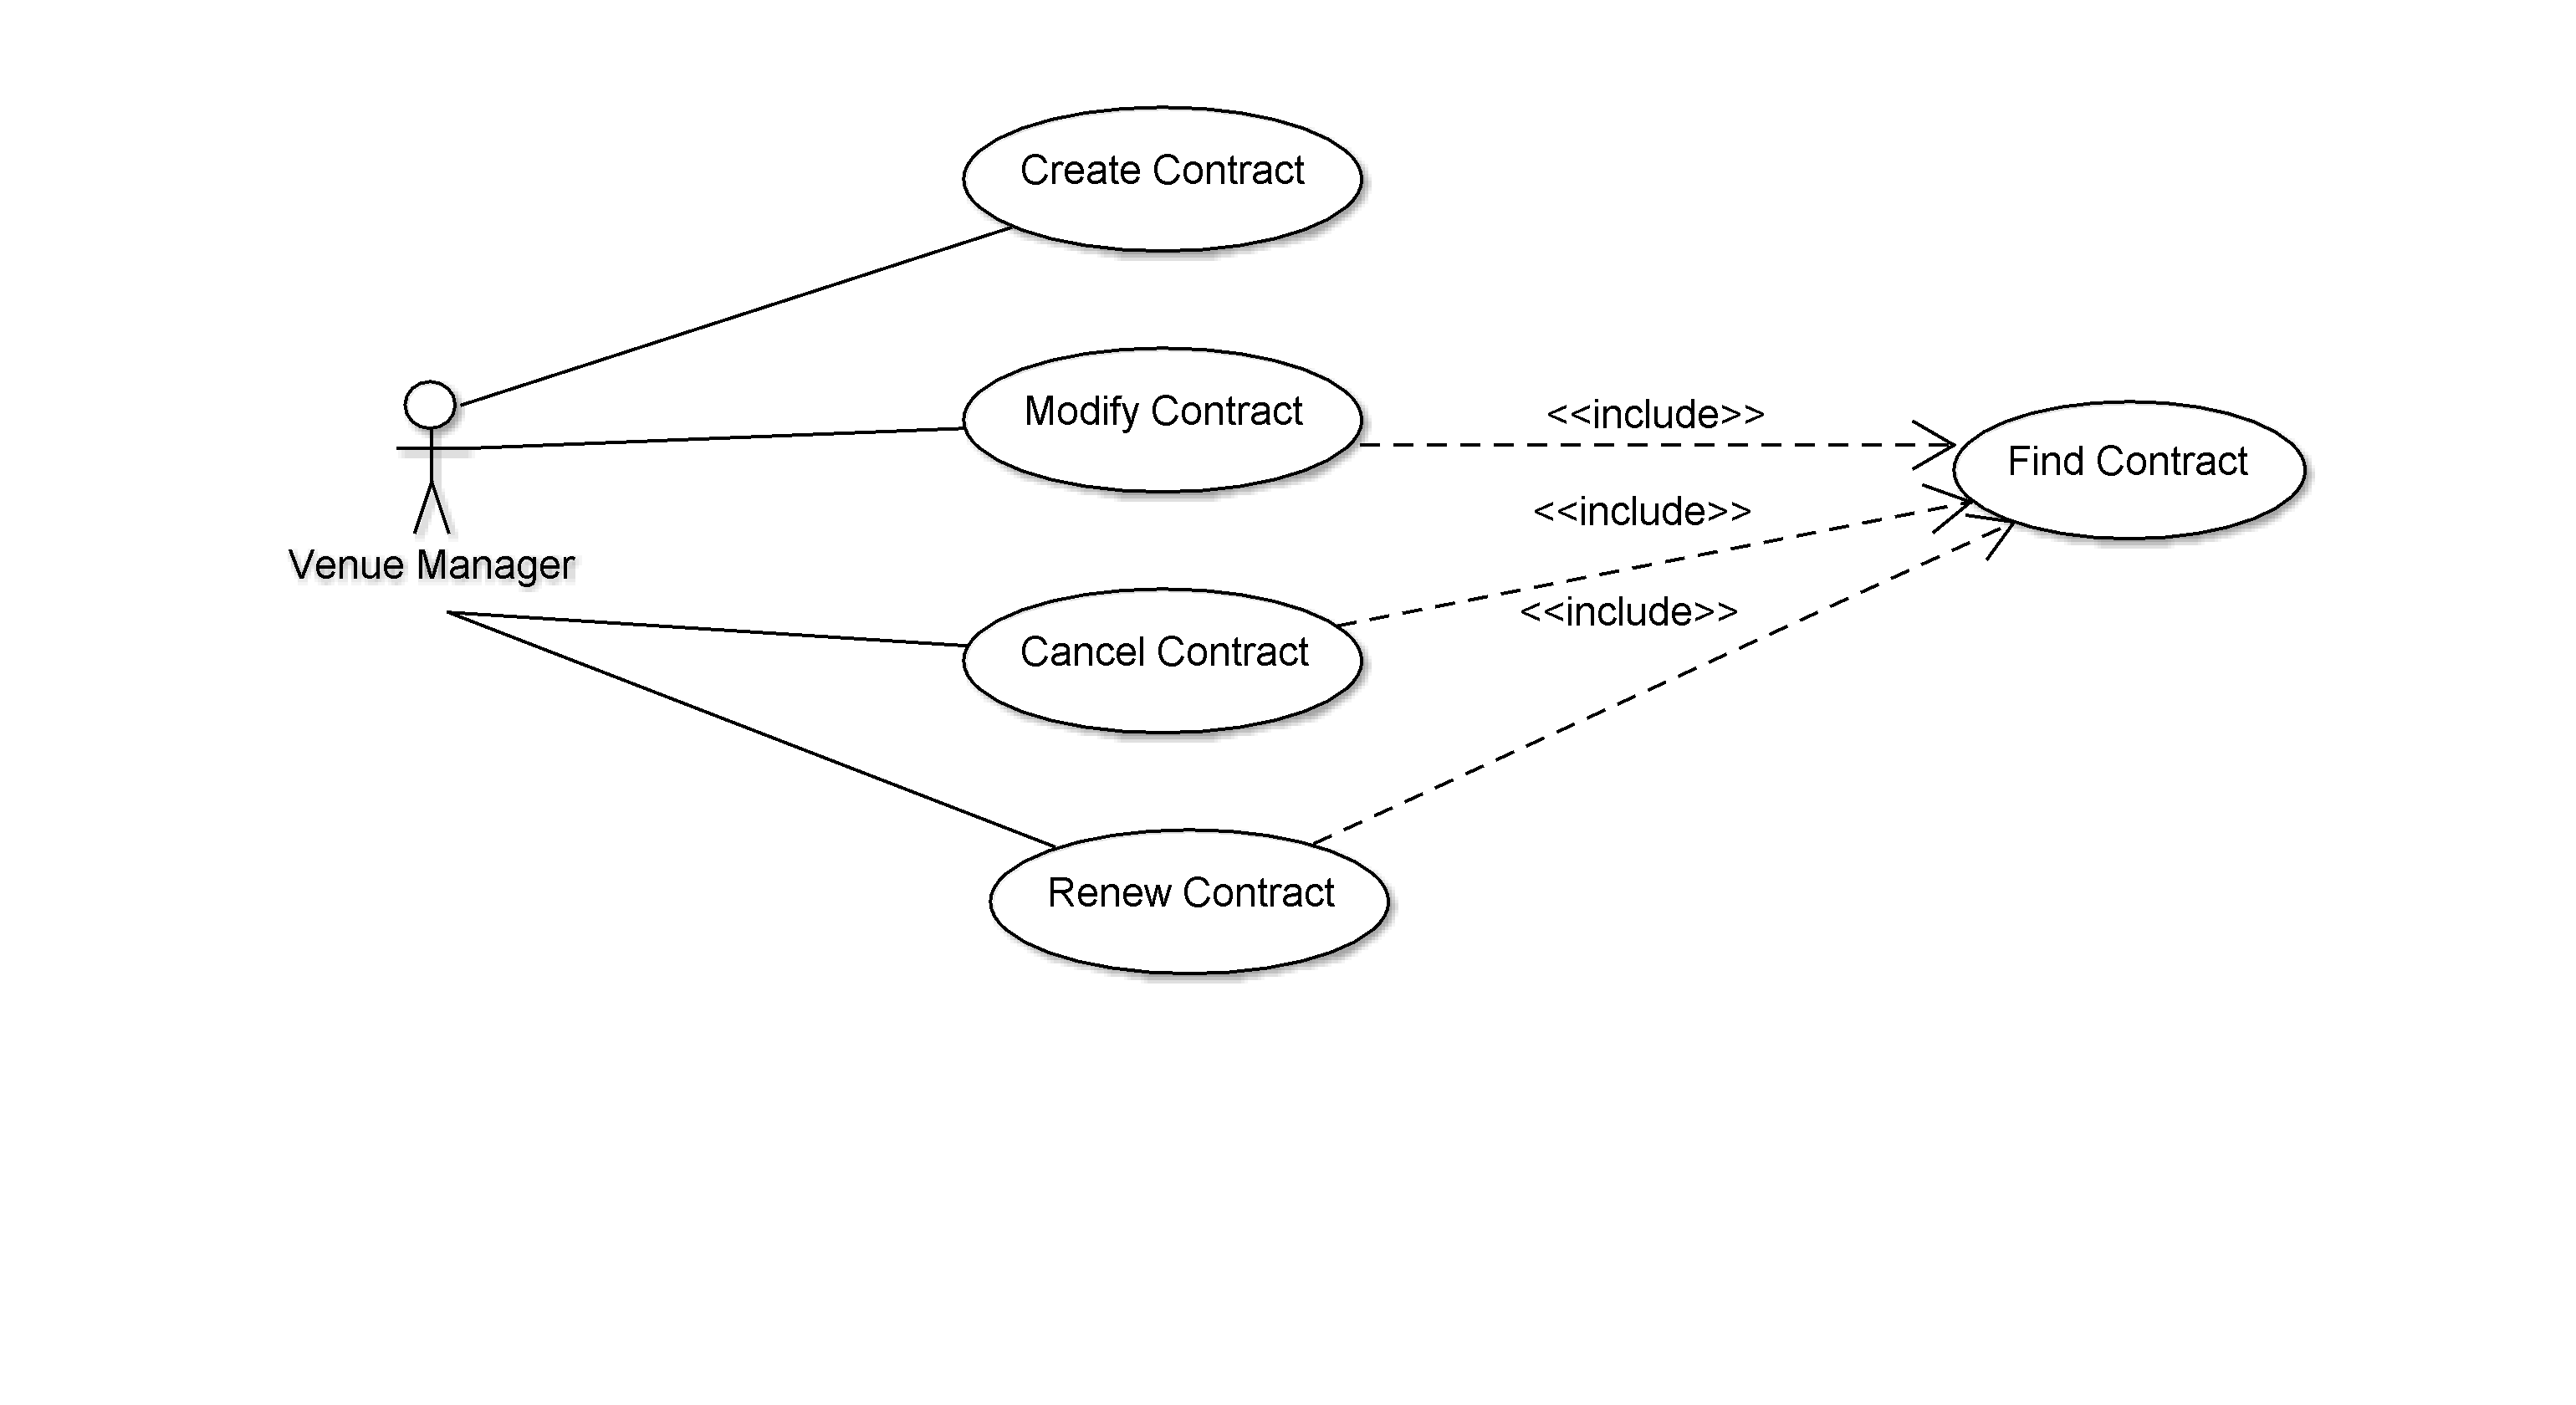
\includegraphics[width=\linewidth]{VenueManagerContractsUsecaseDiagram.png}

Event-related use cases:

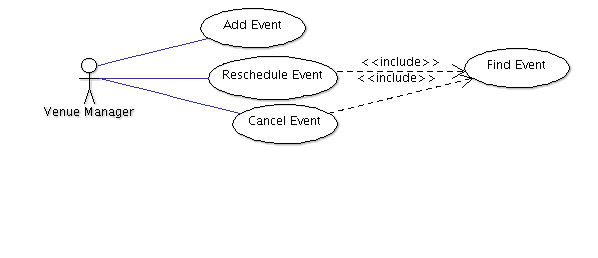
\includegraphics[width=\linewidth]{VenueManagerEventsUsecaseDiagram.png}

Promotion-related use cases:

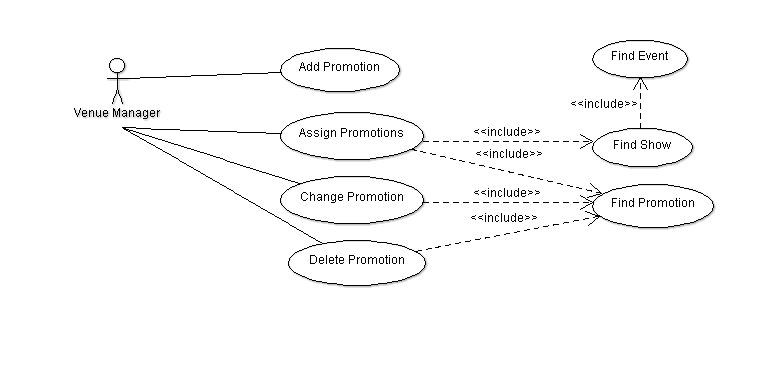
\includegraphics[width=\linewidth]{VenueManagerPromotionsUsecaseDiagram.png}

Show-related use cases:

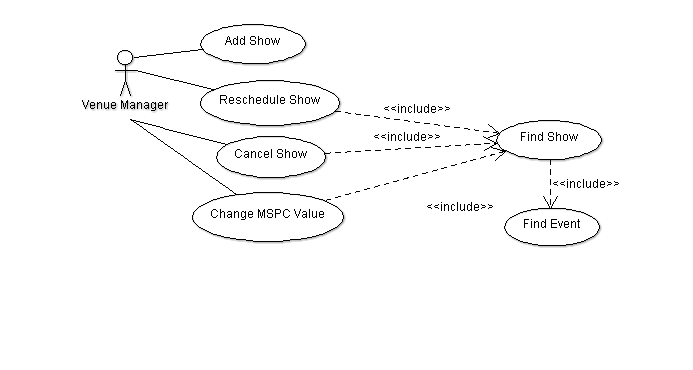
\includegraphics[width=\linewidth]{VenueManagerShowUsecaseDiagram.png}
